\subsection{Teorema de \vank} \label{sec:vank}
Este teorema es considerado como el mas útil a la hora de hacer
identificaciones de grupos fundamentales. Su idea se basa en que si
tenemos un espacio \(X\) y dos subconjuntos \(U,V\) tales que \(X = U
\cup V\), entonces podemos estudiar el grupo \(\pi (X, x_0)\) como un
subgrupo del grupo libre generado por \(\pi (U, x_0)\) y \(\pi (V,
x_0)\). Para obtener un isomorfismo tomamos un cociente adecuado. El
caso mas claro de aplicación se vera que son para las \emph{wedge sum}
en donde este cociente sera trivial. En casos mas generales se vera que
el cociente es de una forma relacionada con la definición de producto
libre. Procedemos para iniciar la definición de estos conceptos.

\begin{definicion}[Producto libre] \label{def:prod-libre}
  Sea \(G_\alpha\) una colección de grupos. El grupo libre \(*_\alpha
  G_\alpha \) consiste como conjunto en todas las cadenas reducidas
  \[ g_1 g_2 g_3 \dots g_m \]
  para \(m \geq 0\) arbitrario tal que todo \(g_i\) pertenece a
  \(G_{\alpha_i}\), \(g_i\) distinto de la identidad de
  \(G_{\alpha_i}\) y índices sucesivos son distintos, ie \(\alpha_i \neq
  \alpha_{i + 1}\). Tomando la identidad como la cadena vacía y como
  operación de grupo la juxtaposicion de cadenas
  \[ (g_1 g_2 \dots g_m ) \cdot (h_1 h_2 \dots h_l) = g_1 g_2 \dots g_m
    h_1 h_2 \dots h_l \]
  en donde se debe reducir la cadena para que términos seguidos no
  pertenezcan al mismo grupo.
\end{definicion}
\begin{acotacion}
  Es claro que la cadena vacía es la identidad. Para ver la inversa de
  una cadena nos basamos en el proceso de reducción. Sea \(g_1 g_2 \dots
  g_m\) una cadena arbitraria, su inversa corresponde a \(g_m^{-1}
  g_{m-1}^{-1} \dots g_1^{-1}\) pues
  \begin{gather*}
    g_1 g_2 \dots g_{m-1} \underbrace{g_m g_m^{-1}}_{= e_{\alpha_m}}
      g_{m-1}^{-1} \dots g_1^{-1} \\
    = g_1 g_2 \dots g_{m-1} g_{m-1}^{-1} \dots g_1^{-1}
  \end{gather*}
  donde la identidad fue removida de la cadena por el requisito de ser
  una cadena reducida. Si este proceso continua iterativamente se
  obtendrá la cadena vacía que es la identidad.

  Por otro lado se nota que no hay requerimiento de que todos los grupos
  participen en todas las cadenas. De hecho, todos los elemento de
  cualquiera de los grupos participantes \(G_\alpha\) pertenecen al
  conjunto de cadenas reducidas como cadenas con \(m = 1\) y índice
  adecuado.
\end{acotacion}
Esta construcción puede considerarse como una alternativa a \(\prod
G_\alpha\) o \(\oplus G_\alpha\) en donde elementos de distintos grupos
no conmuten entre si. Como ejemplo podemos tomar a \(\mathbb Z * \mathbb
Z\) con cada \(\mathbb Z\) con su propio generador, a los cuales
denotaremos por \(a\) y \(b\) respectivamente. Este corresponde al grupo
de la cadenas \(a^{n_1} b^{n_2} a^{n_3} \dots a^{n_m}\) con \(n_i \in
\mathbb Z \). Algo que no es claro sobre este grupo es si
su operación es asociativa, esto lo probaremos en el siguiente teorema
por completitud
\begin{teorema}
  El producto de \(*_\alpha G_\alpha\) es asociativo.
\end{teorema}
\begin{proof}
  Mostrar directamente la asociatividad del producto seria un ejercicio
  de enumerar los casos donde puede ocurrir un reducción de cadena.
  Nosotros seguiremos una vía alternativa dada por \emph{Hatcher} en
  \cite{Hatcher}[sec 1.2] de estudiar la cada posible juxtaposicion como
  una función en el espacio de permutaciones. Sea \(W\) el conjunto de
  cadenas reducidas de \(*_\alpha G_\alpha\) con la cadena vacía
  incluida. Para cada \(g \in G_\alpha\) se define una función asociada
  \(L _g : W \to W\) dada por la ecuación
  \[ L_g \left( g_1 g_2 \dots g_m \right) = g g_1 g_2 \dots g_m \]
  con \(g g_1\) reducido si \(g_1 \in G_\alpha \) para mantener que sea
  una cadena reducida en \(W\). Una propiedad clara es que podemos
  simplificar en \(G_\alpha\) antes o después de asociar \(L\) y no
  afectara el resultado, dicho formalmente sea \(g, g', \hat g \in
  G_\alpha\) con \(\hat g = g \cdot g'\). La asociación \(L_{g \cdot
  g'}\) cumple que \(L _{g \cdot g'} = L_{g} \circ L_{g'}\) pues para una
  cadena arbitraria
  \begin{align*}
    &L_{g \cdot g'} \left( g_1 g_2 \dots g_m \right) \\
    &= (g \cdot g') (g_1 g_2 \dots g_m) \\
    &= (\hat g) (g_1 g_2 \dots g_m) \\
    &= (g (g' (g_1 g_2 \dots g_m))) \\
    &= L_g \circ L_{g'} \left( g_1 g_2 \dots g_m \right)
  \end{align*}
  notando de que en el caso que \(g_1 \in G_\alpha\) se tiene un
  reducción intermedia. Se ve también de todo \(L_g\) con \(g \in
  G_\alpha\) tiene una asociada inversa \(L_{g^{-1}}\) con \(g^{-1} \in
  G_\alpha\), lo cual en consecuencia nos da un mapeo de identidad a
  identidad (por regla de reducción). Por lo anterior tenemos un
  homomorfismo de grupos entre \(G_\alpha\) y \((W \to W, (\circ))\) y
  esto para todo \(\alpha\).
  \begin{align*}
    L: G_\alpha &\longrightarrow P(W) \\
    g &\longmapsto L_g
  \end{align*}

  Podemos de generalizar \(L\) en su primer
  argumento de \(G_\alpha\) con \(\alpha\) arbitrario a todo \(W\). Esto
  se hace por la siguiente formula
  \begin{align}
    \hat L : W &\longrightarrow P(W) \nonumber \\
    g_1 g_2 \dots g_k &\longmapsto L_{g_1} \circ L_{g_2} \circ \dots
    \circ L_{g_k} \label{def:hatL}
  \end{align}
  Una propiedad de \(\hat L\) es que es inyectiva, esto se ve notando
  que las únicas cadenas que mapean bajo \(\hat L\) a la identidad de
  \(P (W)\) corresponden a la cadena vacía o a las identidades de los
  distintos \(G_\alpha\) que por definición no pertenecen a \(W\).

  Ahora podemos ver la asociatividad de \(W\) con la yuxtaposición. Sea
  \(w_1, w_2, w_3 \in W\) tres cadenas tales que \(w_1 (w_2 w_3) \neq
  (w_1 w_2) w_3\). Estudiamos \[\hat L_{w_1 (w_2 w_3)},\ \hat L_{(w_1
    w_2) w_3}\] que por ecuación \eqref{def:hatL} corresponde a la
  composición de varias funciones \(L_g\) con \(g\) elementos de las
  cadenas \(w_1, w_2, w_3\).  No es difícil ver que en ambas expansiones
  participan las mismas funciones \(L_g\) y en el mismo orden. Mas aun,
  dado que la composición en \(P(W)\) es asociativa, nos estaría diciendo
  que
  \[ \hat L_{w_1 (w_2 w_3)} = \hat L_{(w_1 w_2) w_3}\]
  Pero dado que \(\hat L\) es inyectiva, esto implica que \(w_1 (w_2
  w_3) = (w_1 w_2) w_3\). Dada que estas cadenas son arbitrarias,
  estamos diciendo que \(W\) con la yuxtaposición (ie \(*_\alpha
  G_\alpha\)) es asociativo.
\end{proof}

Aquí se utilizo implícitamente un propiedad básica del producto libre
\(*_\alpha G_\alpha\), que si tengo una colección de homomorfismos
\[ \phi_\alpha : G_\alpha \to H \]
con \(H\) un grupo, existe una extensión única
\[ \phi : *_\alpha G_\alpha \to H \]
tal que sigue siendo homomorfismo. En particular, la ecuación que la
define para \(g_1 g_2 \dots g_n \in *_\alpha G_\alpha\) arbitrario es la siguiente
\[
  \phi \left( g_1 g_2 \dots g_n \right) := \phi_{\alpha_1} (g_1)
  \phi_{\alpha_2} (g_2) \dots \phi_{\alpha_n} (g_n)
\]
Para probar que es única, basta notar reducir la cadena no afecta la
imagen bajo \(\phi\) y que esta debe seguir siendo un homomorfismo.

Previo al teorema general, es útil trabajar con una versión reducida del
teorema de \vank por dos razones: es una versión geométricamente
intuitiva y aparece como paso intermedio de la demostración general. En
esta version se trabajara con el siguiente diagrama conmutativo,
\begin{figure}[h]
  \centering
  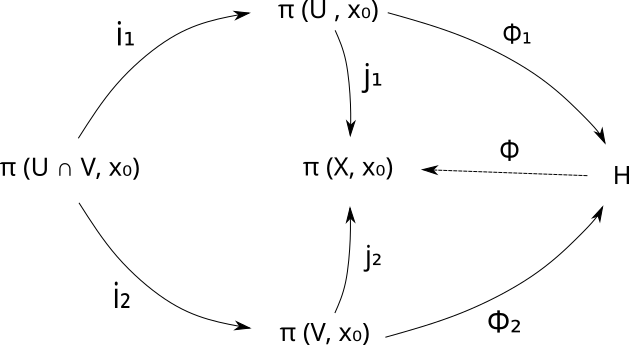
\includegraphics[scale=0.5]{./imagenes/van.png}
\end{figure}
donde \( H = \pi (U, x_0) * \pi (V, x_0)\) el producto libre, \(i_1,
i_2, j_1, j_2\) son los homomorfismos inducidos (sin la notación \(i_*\)
por simplicidad) de las inclusiones correspondientes, \(\Phi_1, \Phi_2\)
son las inclusiones en el grupo libre tomando todo \(\gamma \in \pi (U,
x_0)\) y ver la correspondiente cadena \(\gamma \in H\) y \(\Phi :
\pi(U, x_0) * \pi (V, x_0) \to \pi (X, x_0)\) la extensión de los
homomorfismo \(\Phi_1, \Phi_2\) descrita en el párrafo anterior.

\begin{teorema} \label{thm:vank-especifico}
  Sea \(X = U \cup V\), donde \(U,V\) son conjuntos abiertos de \(X\).
  Supongamos que \(U \cap V\) es arco-conexo y que \(x_0 \in U \cap V\).
  Sea \(j_1\) y \(j_2\) las inclusiones de \(U\) y \(V\) en \(X\)
  respectivamente. Entonces las imágenes de los homomorfismos inducidos
  \[ j_{1,*} : \pi (U, x_0) \to \pi (X, x_0), \quad j_{2,*} : \pi
  (V, x_0) \to \pi (X, x_0) \]
  generan a \(\pi (X,x_0)\).
\end{teorema}
\begin{proof}
  Hemos de probar que para todo arco \(f\) en \(X\) basado en \(x_0\),
  es arco-homotópico a un arco de la forma
  \[ g_1 * g_2 * ... * g_n \]
  donde cada \(g_i\) es un arco en \(X\) basado en \(x_0\) que esta
  contenido completamente en \(U\) o en \(V\).

  Por el lema \ref{thm:lebesgue-number-lema} (numero de Lebesgue),
  existe una subdivisión de \(I\) dada por
  \[ 0 = a_0 < ... < a_n = 1\]
  tal que
  \(f ([a_i , a_{i+1}])\) pertenece completamente a \(U\) o \(V\) para
  todo \(i \in \{1 \dotsc n\}\). Si para para todo \(i\) se cumpliera que
  \(f(a_i) \in U \cap V\) hemos terminado. En caso contrario, de existir
  \(i\) tal que \(f(a_i) \not \in U \cap V\) esto implica que
  \[ f(a_i) \in U \ \veebar \ f(a_i) \in V \]
  Tomando s.p.d.g la primera alternativa, implicaría que
  \[ f(a_i) \in U \implies f([a_{i-1}, a_{i}]) \subset U \ \land \ f([a_i,
    a_{i+1}]) \subset U \]
  análogamente si \(f(a_i) \in V\). Podemos olvidar entonces el valor
  \(a_i\) de la subdivisión y revisar si \(f(a_{i+1}) \in U \cap V\),
  repitiendo este proceso una cantidad finita de veces hasta satisfacer
  la condición.

  Ahora se prueba el teorema en si. Dado \(f\) y \(a_0 < ... < a_n\)
  subdivisión anterior, definamos las funciones
  \[ l_i : [0,1] \to [a_{i-1}, a_{i}] \]
  \[ f_i = f \circ l_i \]
  Es claro que \(\forall i \in \{1 \dotsc n\}, \ f_i (I) \) esta contenida en
  \(U\) o en \(V\). También es claro por simple calculo que se cumple
  la igualdad
  \[ [f] = [f_1] * [f_2] * ... * [f_n] \]
  Pero estos \(\{f_i\}\) no son arcos cerrados basados en \(x_0\) de
  \(\pi (U,x_0)\) o \(\pi (V,x_0)\). Para solucionar esto, nos basamos
  en la arco conexidad de \(U \cap V\), lo que nos permite afirmar que
  para todo \(i \in [1 , n]\) existe
  \[ \alpha_i : I \to U \cap V \]
  \[ \alpha_i (0) = x_0, \quad \alpha_i (1) = f(a_i) \]
  arcos continuos, fijando además \(\alpha_0 \equiv x_0 \equiv \alpha_n
  \). Estos nos permiten construir los arcos
  \[ g_i = \alpha_{i-1} * f_i * \overline{\alpha_i} \]
  los cuales si están basados en \(x_0\), y cuya imagen sigue estando
  contenida en \(U\) o en \(V\). Por simple calculo se ve que
  \[ [g_1] * ... * [g_n] = [f_1] * ... * [f_n] = [f] \]
\end{proof}
\begin{corolario}\label{cor:sobre-van}
  El homomorfismo \(\Phi : \pi (U, x_0) * \pi (V, x_0) \to \pi (X,
  x_0)\) es sobreyectivo.
\end{corolario}
\begin{proof}
  En el final de la demostración anterior, la cadena \(g_1 g_2 \dots
  g_n\) tiene como imagen bajo \(\Phi\) a \([f]\) pues
  \[ \Phi \left( g_1 g_2 ... g_n \right) = [g_1] * [g_2] * ... *
    [g_n] = [f] \]
  Dado que este \([f]\) era un elemento arbitrario de \(\pi \left( X,
    x_0 \right)\), tenemos lo afirmado.
\end{proof}
Uno puede generalizar el teorema anterior para una cantidad arbitraria
de conjuntos \(A_\alpha\) tal que \(X = \bigcup A_\alpha\). La
demostración es la misma, solo tal vez un poco mas difícil de
visualizar. Lo importante de este teorema es el corolario, el cual
utilizaremos en su forma generalizada para probar el teorema general.

\begin{teorema}[\vank]
  Sea \((X, x_0)\) un espacio puntuado tal que exista una familia de
  conjuntos abiertos \(\{A_\alpha\}_{\alpha \in \tau}\) la cual cumpla
  que todo elemento de esta contiene a \(x_0\) y \( X = \bigcup_{\alpha
  \in \tau} A_\alpha\). Si para cada intersección \(A_\alpha \cap
  A_\beta\) es arco-conexa, entonces el homomorfismo
  \[ \Phi : *_\alpha \pi (A_\alpha, x_0) \to \pi (X, x_0) \]
  es sobreyectivo.

  Mas aun, si cada intersección \(A_\alpha \cap A_\beta
  \cap A_\gamma\) con \( \alpha, \beta, \gamma \in \tau\) es arco-conexa,
  entonces el kernel de \(\Phi\) es un subgrupo normal \(N\) de la forma
  \[
    N := N \left( \{ i_{\alpha \beta} (\omega) \overline{i_{\beta
    \alpha} (\omega)} \mid \omega \in \pi \left( A_\alpha \cap A_\beta, x_0
    \right),\ \forall \alpha ,\beta \in \tau \} \right)
  \]
  es decir el subgrupo normal generado por estos elementos y por tanto
  \(\Phi\) induce un isomorfismo \(\pi (X, x_0) \cong *_\alpha \pi
  (A_\alpha, x_0) / N \)
\end{teorema}
Antes de la demostración hablaremos un poco del conjunto \(N\). Las
funciones \(i_{\alpha \beta}, i_{\beta, \alpha}\) corresponden a los
homomorfismos inducidos por la inclusión
\begin{gather*}
  i_{\alpha \beta} : \pi (A_\alpha \cap A_\beta , x_0 ) \longrightarrow \pi (A_\alpha, x_0) \\
  i_{\beta \alpha} : \pi (A_\alpha \cap A_\beta , x_0 ) \longrightarrow \pi (A_\beta, x_0)
\end{gather*}
que pierden su notación \(i_*\) por simplicidad. Notar que
para \(\omega \in \pi (A_\alpha \cap A_\beta ,\ x_0)\) arbitrario
\[ i_{\alpha \beta} (\omega) \overline{i_{\beta \alpha} (\omega)} \in N
  \implies i_{\alpha \beta} (\omega) \cdot N = i_{\beta
\alpha} (\omega) \cdot N \]
con \(i_{\beta \alpha} (\omega) \cdot N\) un elemento de \(*_\alpha \pi
(A_\alpha , x_0) / N\). Lo que lo anterior nos dice es que en \(*_\alpha
\pi (A_\alpha) / N\), las cadenas de \(\pi (A_\alpha \cap A_\beta) / N\)
pueden verse como elementos de \(\pi(A_\alpha) / N\) o \(\pi (A_\beta) /
N\).

También véase que dado el producto en los
grupos cocientes, para \(\omega_1 \omega_2 \) una cadena en \(*_\alpha
A_\alpha\) cumple la ecuación
\[ (\omega_1 \omega_2) N = (\omega_1 N) (\omega_2 N) \]
como elemento del cociente \(*_\alpha A_\alpha / N\). Esto nos permite
modificar puntos finales o iniciales de \(\omega_1, \omega_2\) para
obligar que estos sean elementos de \(\pi (A_1, x_0), \pi (A_2, x_0)\)
respectivamente mediantes operaciones con elementos de \(N\).

Por otro lado, véase que
\[ N \subseteq \text{kernel} \ \Phi \]
pues \(N\) es el menor subgrupo normal de \(*_\alpha A_\alpha\) y los
elementos base de este pertenecen al kernel de \(\Phi\) pues estos son
de la forma
\[ i_{\alpha \beta} (\omega) \ \overline{i_{\beta \alpha} (\omega)} ,
  \ \text{con} \ \alpha,\beta \in \tau,\ \omega \in \pi(A_\alpha \cap
  A_\beta , x_0)\]
y sabiendo como es \(\Phi\) como homomorfismo
\begin{align*}
  \Phi &\left( i_{\alpha \beta} (\omega) \ \overline{i_{\beta \alpha}
          (\omega)} \right) \\
       &= j_{\alpha,*} \left( i_{\alpha \beta} (\omega) \right) *
         j_{\beta,*} \left( \overline{i_{\beta \alpha} (\omega)} \right) \\
       &= j_{\alpha,*} \left( i_{\alpha \beta} (\omega) \right) *
         \overline{j_{\beta,*} \left( i_{\beta \alpha} (\omega) \right)} \\
       &= w * \overline{w} = e
\end{align*}
Con esto
declarado, podemos proceder a la demostración.
\begin{proof}
  En el corolario \ref{cor:sobre-van} ya fue probado que \(\Phi :
  *_\alpha A_\alpha \to \pi (X, x_0)\) es sobreyectivo. Solo nos falta
  caracterizar al kernel de \(\Phi\). Por el tercer teorema del
  isomorfismo \cite{Fraleigh}[sec 34]
  % debo buscar libro de referencia
  si el mapeo inducido por \(\Phi\) a \(*_\alpha A_\alpha / N \to \pi (X,
  x_0)\) es inyectivo y \(N \subseteq \text{kernel}\, \Phi\) entonces \(N =
  \text{kernel} \, \Phi\). Luego podemos aplicar el primer teorema del
  isomorfismo sobre \(\Phi\) para obtener el resultado ya que tenemos
  caracterizado su kernel.

  Seguiremos el esquema de demostracion dado en \cite{Bloom}. Sea \([f]
  \in \pi (X, x_0)\) un elemento arbitrario. Definamos una factorizacion
  de esta como una cadena \([f_1][f_2] ... [f_k] \in *_\alpha \pi
  (A_\alpha, x_0)\) donde
  \begin{enumerate}
  \item Cada \(f_i\) es un camino cerrado en \(A_i\) con punto base \(x_0\)
  \item \(f\) es homotópico a \(f_1 * f_2 * ... * f_k\)
  \end{enumerate}
  Por la sobreyectividad de \(\Phi\) sabemos que existe al menos una
  factorizacion de \([f]\).
  Consideramos que dos factorizaciones son equivalentes si están
  relacionadas por las siguientes dos operaciones o sus inversas:
  \begin{enumerate}
  \item Combinar dos términos adyacentes \([f_i][f_{i+1}]\) a un solo
    termino \([f_i * f_{i+1}]\) si \([f_i],[f_{i+1}] \in \pi
    (A_\alpha)\)
  \item Considerar el termino \([f_i] \in \pi (A_\alpha)\) como
    perteneciente a \(\pi (A_\beta)\) si \(f_i\) es un arco cerrado en
    \(A_\alpha \cap A_\beta\)
  \end{enumerate}
  El primer ``movimiento'' no modifica elementos en \(*_\alpha
  A_\alpha\) pues esta regla es precisamente parte de la noción
  de reducción en el producto libre. El segundo movimiento mantiene al
  elemento de la cadena en la misma clase lateral de \(*_\alpha \pi
  (A_\alpha) / N\) pues si \([f_i] \in \pi (A_\alpha \cap A_\beta)\),
  entonces
  \begin{align*}
    i_{\alpha \beta} \left( [f_i] \right) \overline{i_{\beta \alpha}
      \left( [f_i] \right)} \in N \implies
    &i_{\alpha \beta} \left( [f_i] \right) \cdot N = i_{\beta \alpha}
    \left( [f_i] \right) \cdot N \\
    \iff &[f_i]_{A_\alpha} \cdot N = [f_i]_{A_\beta} \cdot N
  \end{align*}
  y por tanto podemos reemplazar a esta cadena en cualquier posición
  donde aparezca en \(*_\alpha \pi (A_\alpha) / N\) pues si \([x] , [y] \in
  *_\alpha \pi(A_\alpha)\) arbitrarios (partición izquierda y derecha de
  una cadena), se cumple que
  \begin{align*}
    \left( [x] [f_i]_{A_\alpha} [y] \right) \cdot N
    &= \left( [x] \cdot N \right) \cdot \left([f_i]_{A_\alpha} \cdot N
       \right) \cdot \left( [y] \cdot N \right) \\
    &= \left( [x] \cdot N \right) \cdot \left(
      [f_i]_{A_\beta} \cdot N \right) \cdot \left( [y]
      \cdot N \right) \\
    &= \left( [x] [f_i]_{A_\beta} [y] \right) \cdot N
  \end{align*}

  Ahora comenzaremos la demostración de la inyectividad. Supongamos
  que existan dos factorizaciones de \([f]\) en
  \(*_\alpha \pi (A_a, x_0)\)
  \begin{gather*}
    h := [h_1][h_2]\dotsc [h_k] \\
    g := [g _1][g _2]\dotsc [g _l]
  \end{gather*}
  Se probara que se tiene la igualdad como elemento de \(*_a \pi
  (A_\alpha) / N\), ie
  \[ h \cdot N = g\cdot N\]
  Para comenzar, notemos que las cadenas \(h,g\) al ser vistas como
  unión de caminos (ie como imagen bajo \(\Phi\)) cumplen
  \[ [h_1] * [h_2] * \dotsc * [h_k] = [f] = [g _1] * [g _2] * \dotsc * [g _l] \]
  por lo tanto
  \[ h_1 * h_2 * \dotsc * h_k \, \dot \simeq \, g _1 * g _2 * \dotsc *
    g _l \]
  es decir, existe una homotopía en \((X,x_0)\) entre ellas. Denotemos
  a \(F : I \times I \to X\) como dicha homotopía.

  El conjunto \(I \times I\) puede sub-dividirse en una serie de
  cuadriláteros por los puntos
  \[ 0 = s_0 < s_1 < ... < s_m = 1 \]
  \[ 0 = t_0 < t_1 < ... < t_n = 1 \]
  mediante el lema \ref{thm:lebesgue-number-lema} del numero de Lebesgue
  (análogo a lo que se hizo en el teorema
  \ref{thm:levantamiento-homotopico}), los cuales tienen la propiedad de
  que
  \[ \forall (i,j) \in \{0 \dotsc m-1 \} \times \{0 \dotsc n - 1\},
    \ \exists ! \alpha \in \tau,\ F \left( [s_i, s_{i+1}] \times [t_j,
    t_{j+1}] \right) \subseteq A_\alpha \]
  Podemos enumerar los rectángulos generados por estos intervalos como
  \(R_k\) con \(k \in \{1 \dotsc n\cdot m\}\) de izquierda a derecha y
  de abajo hacia arriba. Dada la propiedad anterior, también podemos
  identificar como \( A^{(k)}\) a los conjuntos tales que \(F \left( R_k
  \right) \subseteq A^{(k)} \). Mas aun, podemos modificar ligeramente los
  lados de estos rectángulos de manera que sus vértices estén a lo mas en
  la intersección de tres conjuntos de \(\{A_\alpha\}\).
  \begin{figure}[h]
    \centering 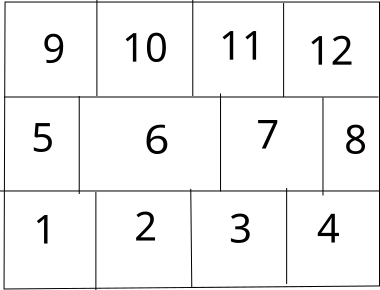
\includegraphics[scale=0.5]{./imagenes/grilla.png}
  \end{figure}

  Definamos la curva \(\gamma_0 (t) := (t, 0)\) que se mueve por el lado
  inferior de \(I \times I\) y cumple que \(F \circ \gamma_0 = \Phi (h)
  \). Análogamente se define una curva \(\gamma_{nm} := (t,1)\) que se
  mueve por el lado superior de \(I \times I\) y que cumple \(F \circ
  \gamma_{nm} = \Phi (g)\). Consideremos a las curvas \(\gamma_k\) como
  aquellas que separen a los rectángulos \(R_1 \dots R_k\) del resto y que
  vayan desde el borde izquierdo al borde derecho. Es claro que
  \[ \forall k,\ F \circ \gamma_k (0) = x_0 = F \circ \gamma_k (1) \]
  es decir, estos son arcos cerrados de \(x_0\). También se ve que
  podemos pasar del arco \(\gamma_k\) al arco \(\gamma_{k+1}\) por la
  homotopía de la linea recta \(\Gamma_k\) contenida en el rectángulo
  \(R_k\), pues el espacio \(I \times I\) es convexo. Por tanto \(F \circ
  \Gamma_k\) es una homotopía entre \(F \circ \gamma_k\) e \(F \circ
  \gamma_{k+1}\).

  Por otro lado, llamemos a las esquinas de los rectángulos \(R_k\)
  vértices. Para cada vértice \(v\) tal que \(F (v) \neq x_0\), sea
  \(g_v\) el arco desde \(x_0\) hasta \(F(v)\). Podemos elegir que
  \(g_v\) tenga su imagen contenida en la intersección de a lo mas tres
  conjuntos \(A_\alpha\) pues por hipótesis, estas intersecciones son
  arco-conexas y contienen a \(x_0\).

  Para todo \(k \in \{1 \dots mn\}\), la curva \(F \circ \gamma_k\)
  tiene una factorizacion por el siguiente procedimiento: Construimos
  una sucesión de arcos (no necesariamente cerrados)
  \[ f_1^{(k)} * f_2^{(k)} * ... * f_l^{(k)} = F \circ \gamma_k \]
  separando a \(F \circ \gamma_k\) en intervalos de manera que queden
  alineados a los vértices de los rectángulos. Esto es un
  procedimiento análogo al utilizado en el teorema
  \ref{thm:vank-especifico}. Entre cada elemento \(f_i^{(k)}\)
  introducimos los caminos \(\bar g _v , g_v\) de ser necesario para
  obligar a que se cumpla
  \[\bar g _v * f_i^{(k)} * g_v \in \pi (A_\alpha, x_0)\]
  Así obteniendo una factorizacion de \([F \circ \gamma_k]\) para todo
  \(k\) tomando las clases de equivalencias (homotópicas) de los
  elementos anteriores y usándolas para formar las cadenas respectivas
  en \(*_\alpha \pi (A_\alpha, x_0)\).

  Esta factorizacion depende de cierto parámetros, puesto que \(\gamma_k\)
  tiene su imagen en las aristas de los rectángulos y potencialmente
  podría darnos varias factorizaciones con elementos en distintos \(\pi
  (A_\alpha)\). Sin embargo, debemos recordar que estas factorizaciones
  seria equivalentes bajo el movimiento dos de factorizaciones descrito
  anteriormente. Mas aun, dado que \(h\) e \(g\) pueden tener
  potencialmente distinta cantidad de elementos en sus cadenas, es
  necesario hacer aparecer elementos extra entre medio mediante el
  segundo movimiento de factorizaciones.

  Por ultimo, notamos que las factorizaciones de \([F \circ \gamma_k]\) e
  \([F \circ \gamma_{k+1}]\) son equivalentes. Esto es debido a la
  homotopía \(F \circ \Gamma_k\), ya que esta solo cambia las curvas en el
  segmento contenido en el rectángulo \(R_k\). Denotaremos a \([a_k,
  a_{k+1}] \subseteq I\) al intervalo tal que
  \[F \circ \gamma_k \, ([a_k , a_{k+1}]) \subseteq R_k\]
  y fijamos un elemento \([f_a^{(k)}]\) de la factorizacion de \([F
  \circ \gamma_k]\) como aquel que le corresponde la seccion del argumento
  \([a_k , a_{k+1}]\). La factorizacion de \([F \circ \gamma_k]\) en
  general correspondera a
  \[ [f_1^{(k)}] [f_2^{(k)}] ... [f_a^{(k)}] ... [f_m^{(k)}] \]
  Por otra parte, la factorizacion de \([F \circ \gamma_{k+1}]\) es
  analoga con su propio elemento \([f_a^{(k+1)}]\) con imagen en
  \(A^{(k)}\) y misma cantidad de elementos.
  \[ [f_1^{(k+1)}] [f_2^{(k+1)}] ... [f_a^{(k+1)}] ... [f_m^{(k+1)}] \]
  Dado que la homotopia \(F \circ \Gamma_k\) solo varia en \(R_k\), se
  tiene que el unico elemento de las imagenes de las cadenas que varian
  son aquellos que pertenece a \(\pi (A^{(k)})\) en el intervalo \([a_k,
  a_{k+1}]\), por lo tanto
  \[ f_a^{(k)} \dot \simeq f_a^{(k+1)} \]
  lo que a su implica la igualdad
  \[ [f_a^{(k)}] = [f_a^{(k+1)}]\]
  por lo que podemos reemplazar los valores en las cadenas. Probando asi
  que son iguales y por tanto equivalentes.

  Luego, dado que \(h\) y \(g\) son factorizaciones de \([F \circ
  \gamma_0]\) e \([f \circ \gamma_{nm}]\) respectivamente y que las
  factorizaciones de \([F \circ \gamma_k]\) son todas equivalentes para
  todo \(k\), se obtiene \(h\) y \(g\) son equivalentes. Por lo tanto
  ambas pertenecen a la misma clase lateral de \(*_\alpha \pi (A_\alpha ,
  x_0)\). Por la arbitrariedad de \([f] \in \pi (X, x_0)\) e \(g,h \in
  *_\alpha \pi (A_\alpha)\), se tiene que el mapeo inducido por \(\Phi\)
  en \(*_\alpha \pi (A_\alpha) / N \to \pi (X,x_0)\) es inyectivo.
\end{proof}
\begin{corolario} \label{cor:vank-trivial}
  Si \(\bigcap_{\alpha \in \tau} A_\alpha \) tiene grupo fundamental
  trivial, entonces
  \[ *_\alpha \pi (A_\alpha , x_0) \simeq \pi (X, x_0) \]
\end{corolario}

\begin{corolario}[Preservación del co-producto bajo \(\pi\)]
  \label{cor:vank-coproducto}
  Sea \(x_0 \in X, \ y_0 \in Y\), si existen \(U_x \subset X, \ U_y
  \subset Y\) vecindades simplemente conexas (contractibles) a \(x_0,
  y_0\) respectivamente, entonces el wedge-sum \((X \vee Y , \{x_0 ,
  y_0\})\) tiene grupo fundamental \(\pi (X, x_0) * \pi (Y, y_0)\).
\end{corolario}
\begin{proof}
  Definamos dos nuevos conjuntos:
  \begin{gather*}
    A_x := (X \vee U_y / {x_0 \simeq y_0}) \\
    A_y := (Y \vee U_x / {x_0 \simeq y_0})
  \end{gather*}
  Dada que \(U_x, U_y\) son contráctiles, se tiene que \(A_x, A_y\)
  poseen los mismos tipos homotopicos que \(X, Y\) respectivamente, ie
  \begin{gather*}
    \pi (A_x , x_0) = \pi (X, x_0) \\
    \pi (A_y , y_0) = \pi (Y, y_0)
  \end{gather*}
  Además estos conjuntos cumplen las siguiente ecuaciones
  \begin{gather*}
    A_x \cup A_y = (X \vee Y / \{ x_0 \sim y_0\}) \\
    A_x \cap A_y = (U_x \vee U_y / \{ x_0 \sim y_0\})
  \end{gather*}
  Otra vez por ser \(U_x, U_y\) contráctiles, el grupo fundamental
  \(\pi (A_x \cap A_y, x_0)\) es trivial y por tanto podemos aplicar el
  corolario \ref{cor:vank-trivial} para obtener que
  \[ \pi (X \vee Y, x_0) = \pi (X, x_0) * \pi (Y, y_0) \]
\end{proof}

\begin{ejemplo}[Espacio ``figura 8'']
El espacio ``figura 8'' en el diagrama es homotopicamente equivalente a
la wedge-sum \(S^1 \vee S^1\).
  \begin{figure}[h]
    \centering 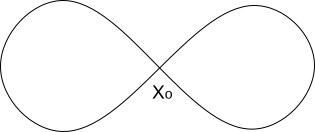
\includegraphics[scale=0.5]{./imagenes/figura8.png}
    \caption*{Espacio figura 8}
  \end{figure}
  Es trivialmente cierto que el conjunto \(\{x_0\}\) es arco-conexo y
  hay inyecciones dos canónicas de \(S^1\) a \(S^1 \vee S^1\). Además es
  cierto que \(x_0\) posee vecindades contráctiles en \(S^1\), pues este
  es homeomorfo a \([0,1]/0 \simeq 1\) y es cosa de tomar un intervalo
  pequeño de \(x_0\). Por tanto podemos aplicar el corolario
  \ref{cor:vank-coproducto} para decir que el grupo fundamental de
  \(\left( S^1 \vee S^1 , x_0 \right) \) es \(\pi \left( S^1 , x_0 \right)
  * \pi \left( S^1 , x_0 \right) \).
\end{ejemplo}

El producto libre de grupos \(*_\alpha G_\alpha\) es en la categoría
\(\mathcal{Grp}\) el co-producto categórico. Una consecuencia
de \vank es que el functor \(\pi : \mathscr{HoTop}_* \to \mathscr{Grp}\)
preserva \emph{algunos} co-productos, en particular aquellos
co-productos cuyos espacios bases tengan vecindades simplemente conexa en los
puntos de origen.

seria interesante ver algún ejemplo de un co-producto que no se preserva
bajo \(\pi\). Para esto solo debemos ver algun espacio que no tenga
vecindades simplemente conexas para todo punto\footnote{no sea semi localmente
simplemente conexo}. Para esto consideramos el espacio ``Hawaian earring''
\begin{figure}[h]
  \centering
  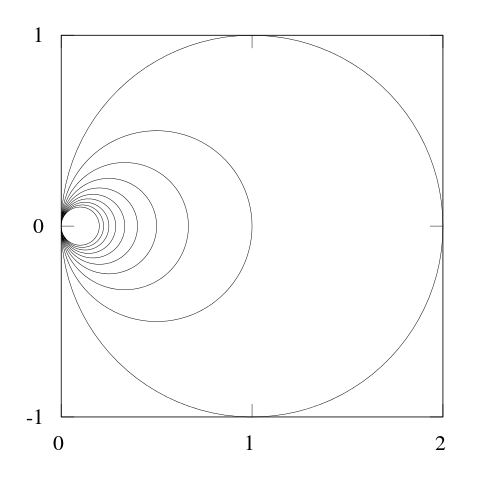
\includegraphics[scale=0.3]{./imagenes/480px-Hawaiian_Earrings.svg.png}
  \caption*{Hawaian earring}
\end{figure}
el cual es la unión de \(S^1\) de radio \(1 / n\) centrados en
\((1/n, 0)\) para todo \(n \in \mathbb N\). Si consideramos a \(x_0\)
como la intersección de todos los círculos, para cualquier vecindad
(como vecindad restringida de \(\mathbb R ^2\)) esta siempre contendrá a
algún \(S^1\) de radio \(1 / {n_0}\) para \(n_0\) suficientemente
grande. Luego este espacio no sera simplemente conexo, pues \(S^1\) no
es contractible a un punto un punto. Luego no podemos concluir mediante
\vank que
\[ \pi (X \vee X , x_0) = \pi (X, x_0) * \pi (X, x_0)\]
cuando \(X\) es el ``Hawaian earring''.

\begin{ejemplo}[Botella de Klein]
  La botella de Klein \(K\) puede presentarse como un cociente en el
  espacio \(I \times I\) representada por el siguiente diagrama.
  \begin{figure}[h]
    \centering 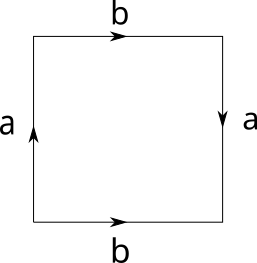
\includegraphics[scale=0.5]{./imagenes/klein.png}
    \caption*{Conjunto \(K\)}
  \end{figure}
  Este espacio puede ser cubierto por los siguientes conjuntos \(U,V\).
  \begin{figure}[h]
    \centering
    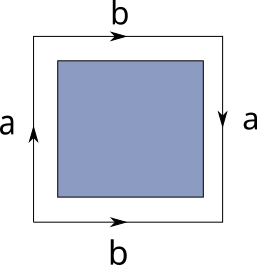
\includegraphics[scale=0.5]{./imagenes/kleinU.png}
    \hspace{3mm}
    
\includegraphics[scale=0.5]{./imagenes/kleinV.png}
    \hspace{3mm}
    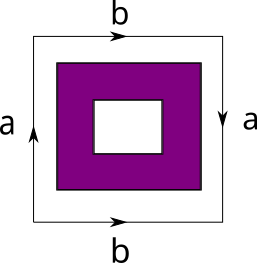
\includegraphics[scale=0.5]{./imagenes/kleinUV.png}
    \caption*{Conjuntos \(U\), \(V\) y \(U \cap V\) respectivamente}
  \end{figure}
  Es claro que \(K = U \cup V\). Elegíamos un punto \(x_0 \in U \cap V\).
  El grupo fundamental \(\pi \left( U , x_0 \right) \) es trivial porque
  este conjunto es convexo y todos los caminos son homotópicas a la
  identidad. El grupo fundamental de \(\pi (V, x_0)\) es isomorfo a
  \(\pi (V, y_0)\) con \(y_0\) el vértice (que identificado es único) de \(I
  \times I\), esto pues el espacio \(V\) es arco-conexo. Estudiando
  \(\pi (V, y_0)\), es claro que \(V\) es homotopicamente equivalente al
  espacio generado por la curvas \(a\) y \(b\) con punto común \(y_0\),
  es decir .
  \[ \pi (V, x_0) \cong \pi (V, y_0) \cong \pi (S^1 \vee S^1, y_0) =
    \mathbb Z * \mathbb Z \]
  tomando a \(a,b\) como generadores.

  Para aplicar \vank debemos estudiar el espacio \(N\). Notese que el
  espacio \(U \cap V\) es homotopicamente equivalente a una curva
  \(\gamma\) contenida en \(U \cap V\) que de una vuelta completa.
  \(\gamma\) es homeomorfa a \(S^1\) y por tanto el
  \[\pi (U \cap V, x_0) \cong \pi (S^1) = \mathbb Z \]
  con \(\gamma\) el generador de este. Debemos estudiar los
  homomorfismos inducidos por la inclusión
  \[ i_{u v} : \pi (U \cap V , x_0) \longrightarrow \pi (U, x_0) \]
  \[ i_{v u} : \pi (U \cap V , x_0) \longrightarrow \pi (V, x_0) \]
  y \(  \pi (U \cap V , x_0) = \langle {[\gamma]} \rangle \). Por
  simple calculo se ve que
  \begin{gather*}
    i_{u v} ([\gamma]) = [\gamma]_{U} = e \in \pi \left( U, x_0 \right)
    \\
    i_{v u} ([\gamma]) = [\gamma]_{V} \in \pi \left( V, x_0 \right)
  \end{gather*}
  con \(e \in \pi \left( U, x_0 \right)\) la identidad de ese grupo y el
  único elemento posible en el recorrido. Véase que \([\gamma]_V\) es
  equivalente homotopicamente a \([a * b * a * b^{-1}]\) por la proyección
  radial desde el centro de \(I \times I\) hacia el borde.
  \begin{figure}[h]
    \centering 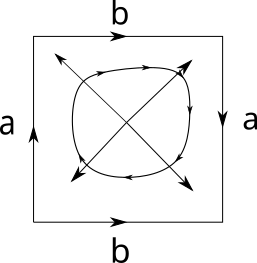
\includegraphics[scale=0.5]{./imagenes/radial.png}
  \end{figure}
  Luego el conjunto \(N\) corresponde al normalizador
  \[ N \{ [a] [b] [a] [b^{-1}]\}\]
  donde este conjunto corresponde simplemente \(\{ [a] [b] [a]
  [b^-1]\}\) con la yuxtaposición como operación, es decir no tiene
  elementos extra de \(\pi (U,x_0) * \pi (V, x_0)\). Luego \vank nos
  dice que se tiene los siguientes isomorfismos
  \[ \pi (K, x_0) \cong \left( \pi (U, x_0) * \pi (V, x_0) \right)
      /_{\{[a] [b] [a] [b^{-1}]\}} = \langle {a , b} \rangle
      /_{\{[a] [b] [a] [b^{-1}]\}}\]
  donde este ultimo puede presentarse como las cadenas generadas por
  \(a,b\) con \(a * b * a * b^{-1} \) reducido o removido por ser la
  identidad, ie
  \[ \langle a,b \rangle /_{abab^{-1} = e} \]
\end{ejemplo}

\subsubsection{Pushout}
Además del producto y el co-producto existen otras estructuras
categóricas que también tienen propiedades universales. Una de interés
en visión de el teorema \vank es la de un pushout. Veremos a
continuación una definición
\begin{definicion}[Pushout]
Sea \(\mathscr{C}\) una categoría. Sean \(X,Y,Z\) objetos en
\(\mathbf{Obj}(\mathscr{C})\) y \(f : Z \to X , g : Z \to Y\) morfismos
en \(\mathscr{C}\). El pushout de \(f,g\) corresponde a una tripleta
\((P, i_1, i_2)\) donde \(P\) es un objeto, \(i_1 : X \to P ,\ i_2 : Y
\to P\) son morfismos de la categoría \(\mathscr{C}\) tales que
\[ i_1 \circ f = i_2 \circ g\]
y que estos sean universales. Esto es, que si existe una tripleta \((Q,
j_1, j_2)\) con \(Q\) un objeto y \(j_1 : X \to Q,\ j_2 : Y \to Q\)
tales que el diagrama conmute, ie
\begin{gather*}
  j_1 \circ f = j_2 \circ g
\end{gather*}
entonces existe un morfismo \(u : P \to Q\) tal que
\[ j_2 = u \circ i_2, \quad j_1 = u \circ i_1 \]
En resumen, el siguiente diagrama conmuta en todo posible camino
\begin{figure}[h]
    \centering 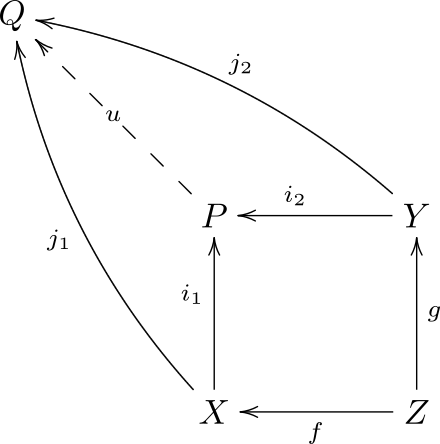
\includegraphics[scale=1]{./imagenes/pushout.png}
\end{figure}
\end{definicion}

En la categoría \(\mathscr{Top}_*\) o \(\mathscr{HoTop}_*\) los espacios
adjuntos son los pushout de morfismos dado por la inclusión. Formalmente,
si \(A,B,C\) son espacios topológicos donde \(f : A \to B \) es una
función inclusión y \( g : A \to C \) es una función continua, el
espacio
\[ B \cup_{g} C := B \sqcup C / \{g(A) \sim f(A)\} \]
junto con las inclusiones correspondientes al co-producto es el pushout
de \( (A, f , g) \).

En la categoría \(\mathscr{Grp}\), el pushout general es el llamado
producto libre con amalgamación. Formalmente, si \(F,G,H\) son grupos
con morfismos \(\psi : F \to G ,\ \phi : F \to H\), su pushout sera el
grupo
\[ G * H / \text{Norm}\{ \phi(f) \psi(f)^{-1} = e , \forall f \in F\}\]
con las respectivas inclusiones al co-producto (modulo clases de
equivalencia).

Podemos re-interpretar el teorema de \vank mediantes pushouts. El
teorema general nos dice que el grupo fundamental de un espacio adjunto
\(A \cup_f B\) con \(i_{a,b} : A \cap B \to A, i_{b,a} : A \cap B \to B
\) \emph{ambas} inclusiones y \(A \cap B\) un espacio arco-conexo,
corresponde a el grupo libre con amalgamación
\[\pi (A, x_0) * \pi (B , x_0) / N \{i_{a,b,*} (f)
\overline{i_{b,a,*} (f)} = e , \forall f \in \pi (A \cap B)\},\ x_0 \in
A \cap B \]
Es decir, el functor \(\pi\) preserva pushouts dados por funciones
inclusión de \(\mathscr{HoTop}_*\) a pushout de \(\mathscr{Grp}\)
(recordando que estos elementos pierden su notación \(i_*\) por
simplicidad).
\begin{figure}[h]
  \centering 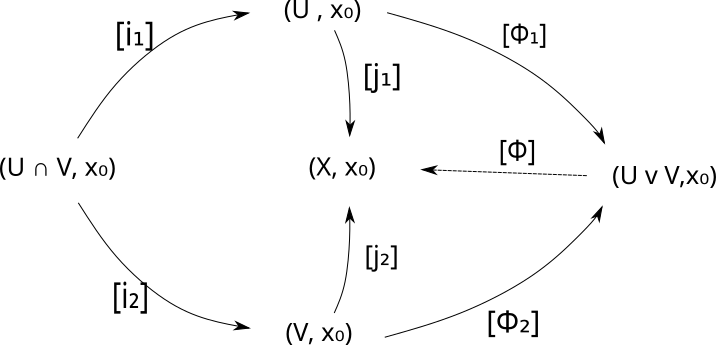
\includegraphics[scale=0.4]{./imagenes/pushoutHotop.png}
  \caption*{\(H = (U \cup_{i_1} V, {x_0, y_0})\)}
  \caption*{\(\pi (H) = U \vee V/ \text{N}\{i_{a,b}(\gamma)\overline{i_{b,a}}
    (\gamma) \mid \gamma \in \pi(U \cap V)\})\)}
\end{figure}

Por ultimo, cabe notar de que existen generalizaciones del teorema
\vank donde las hipótesis de arco-conexidad (y conexidad) no participen.
Estos resultados también se presentan como la preservación de alguna
estructura que preserve una propiedad universal en una categoría
adecuada. Se guía a revisar la referencia \cite{brown} para los
interesados en dichas construcciones.
